\documentclass[aspectratio=169,11pt]{beamer}

% ---------- Theme ----------
\usetheme[numbering=fraction]{metropolis}
\setbeamertemplate{caption}{\raggedright\insertcaption\par}

% ---------- Packages ----------
\usepackage[T1]{fontenc}
\usepackage{lmodern}
\usepackage{amsmath,amssymb}
\usepackage{booktabs}
\usepackage{graphicx}
\usepackage{array}
\usepackage{hyperref}
\usepackage{caption}

% ---------- Metadata ----------
\title{Model Compression and Efficiency Optimisation\\for Edge Deployment}
\subtitle{Diploma Seminar 2 --- Presentation 2\\Results and Evaluation}
\author{Hubert Jaczynski}
\institute{
  Warsaw University of Technology\\
  \vspace{1mm}
  \footnotesize Supervisor: PhD. Maria Ganzha
}
\date{Warsaw, 2026}

% ---------- Helpers ----------
\newcommand{\noteTime}[1]{\note{\textbf{Timing:} #1}}
\newcommand{\metric}[2]{\textbf{#1} {\footnotesize #2}}
\newcommand{\ok}{\textit{done}}
\newcommand{\pending}{\textit{pending}}
\newcommand{\blocked}{\textit{blocked}}

\begin{document}

\maketitle
\noteTime{0:00--0:30. Say this is not a new methodology deck; it is a results and evaluation update.}

% -----------------------------
\begin{frame}{Thesis reminder}
\begin{itemize}
  \item The thesis studies \textbf{model compression and efficiency optimisation} for real-time object detection.
  \item The practical target is edge-oriented deployment, where accuracy alone is not enough.
  \item The central comparison is between detector families and compression variants under one benchmark workflow.
  \item This presentation focuses on the current results, not the full literature review.
\end{itemize}

\vspace{3mm}
\textbf{Question behind the thesis:} which detector and compression path gives the best accuracy--latency trade-off on constrained hardware?
\noteTime{0:30--1:15. Set context for people who do not remember Presentation 1.}
\end{frame}

% -----------------------------
\begin{frame}{Why this problem matters}
\begin{itemize}
  \item Object detectors are often evaluated mainly by COCO mAP, but deployment is constrained by more than accuracy.
  \item A detector may be accurate but unsuitable if it is too slow, too large, or too expensive to run continuously.
  \item Edge-like systems usually have:
  \begin{itemize}
    \item strict latency and throughput limits,
    \item limited GPU memory or accelerator memory,
    \item device-specific runtime support,
    \item power and thermal constraints.
  \end{itemize}
  \item Therefore, the thesis treats detection as an \textbf{accuracy--latency--runtime} problem.
\end{itemize}
\noteTime{1:15--2:10. Give a concrete example: camera stream, robot, or smart monitoring pipeline.}
\end{frame}

% -----------------------------
\begin{frame}{Research objective}
\begin{block}{Main objective}
Identify which compression and efficiency optimisation techniques, or combinations of techniques, provide the best accuracy--latency--size trade-off for real-time object detection on constrained hardware.
\end{block}

\begin{itemize}
  \item The work compares published COCO-trained detectors under controlled local measurements.
  \item It separates architecture choice from runtime/precision choice.
  \item It then prepares the ground for token reduction, pruning, and compression-order experiments.
\end{itemize}
\noteTime{2:10--3:00. This is the thesis anchor; keep it precise.}
\end{frame}

% -----------------------------
\begin{frame}{Research questions}
\begin{enumerate}
  \item Which detector family gives the best accuracy--latency trade-off before compression?
  \item How much speed can be gained from FP16 and TensorRT INT8 PTQ?
  \item Do newer YOLO variants behave differently from YOLOv8 under the same precision changes?
  \item Does a transformer-style detector need token-level compression to become competitive in latency?
  \item Which compression sequence should be explored next: quantisation first, token reduction first, or pruning first?
\end{enumerate}
\noteTime{3:00--4:00. These questions map directly to the result slides later.}
\end{frame}

% -----------------------------
\begin{frame}{Working hypotheses}
\begin{itemize}
  \item \textbf{H1:} INT8 PTQ should reduce latency more strongly than FP16, but with a measurable mAP drop.
  \item \textbf{H2:} the mAP drop from compression is architecture-dependent, not a fixed percentage.
  \item \textbf{H3:} RF-DETR should provide a strong accuracy anchor, but FP16 alone will not be enough for low-latency deployment.
  \item \textbf{H4:} newer YOLO variants should shift the baseline Pareto curve before any extra pruning or token reduction is applied.
\end{itemize}
\noteTime{4:00--5:00. These are working hypotheses, not final claims yet.}
\end{frame}

% -----------------------------
\begin{frame}{Scope and assumptions}
\begin{itemize}
  \item Main dataset: COCO 2017 validation.
  \item Main hardware: NVIDIA GeForce RTX 3070 Ti with 8 GB VRAM.
  \item Main batch size: 1, because real-time detection is usually latency-sensitive.
  \item Compression currently evaluated: FP16 inference and INT8 PTQ for YOLO through TensorRT.
  \item Compression still planned: RF-DETR/Swin token reduction, RF-DETR INT8 export, light structured pruning.
  \item The results are preliminary thesis results, not final deployment claims for every edge device.
\end{itemize}
\noteTime{5:00--5:50. This keeps the scope honest and prevents overclaiming.}
\end{frame}

% -----------------------------
\begin{frame}{Model families in the benchmark}
\small
\begin{tabular}{>{\raggedright\arraybackslash}p{0.25\textwidth}>{\raggedright\arraybackslash}p{0.28\textwidth}>{\raggedright\arraybackslash}p{0.38\textwidth}}
\toprule
\textbf{Family} & \textbf{Representative} & \textbf{Reason for inclusion}\\
\midrule
Detection transformer & RF-DETR Medium & High COCO accuracy and transformer-style detection pipeline.\\
Hierarchical ViT & Swin-T Mask R-CNN & Planned comparison for windowed/hierarchical attention.\\
YOLO baseline & YOLOv8s, YOLOv8m & Mature dense-detector baseline with strong tooling.\\
Newer YOLO & YOLO26s, YOLO26m & Newer Ultralytics family requested for the thesis comparison.\\
\bottomrule
\end{tabular}

\vspace{4mm}
\textbf{Design idea:} compare models that represent different architecture choices, then apply comparable compression axes.
\noteTime{5:50--6:50. Mention that Swin remains part of the design even though it is currently blocked locally.}
\end{frame}

% -----------------------------
\begin{frame}{Compression axes}
\begin{itemize}
  \item \textbf{Precision reduction:} FP32 baseline, FP16 inference, INT8 post-training quantisation.
  \item \textbf{Token reduction:} planned for RF-DETR and Swin, where attention operates over visual tokens.
  \item \textbf{Structured pruning:} planned for YOLO-style models, where channel/filter pruning maps better to hardware.
  \item \textbf{Ordering:} later ablations will compare whether quantisation before pruning/token reduction is better than the reverse.
\end{itemize}


\noteTime{6:50--7:50. This slide connects the results to the full thesis plan.}
\end{frame}

% -----------------------------
\begin{frame}{What changed since Presentation 1}
\begin{itemize}
  \item The benchmark workflow is now operational on the local RTX 3070 Ti.
  \item COCO 2017 validation data and annotations are available locally.
  \item RF-DETR Medium has completed FP32 and FP16 evaluation.
  \item YOLOv8s/m and YOLO26s/m have completed FP32, FP16, and TensorRT INT8 PTQ evaluation.
  \item Swin-T Mask R-CNN is still queued, but native Windows/OpenMMLab setup is the current blocker.
\end{itemize}

\vspace{2mm}
\textbf{Main point:} the first full evaluation already gives a clear accuracy--latency picture for transformer and YOLO-style detectors.
\noteTime{0:30--1:40. Keep this short; the audience already heard the motivation and methodology earlier.}
\end{frame}

% -----------------------------
\begin{frame}{Evaluation protocol}
\begin{columns}[T,onlytextwidth]
\begin{column}{0.50\textwidth}
\textbf{Data}
\begin{itemize}
  \item Dataset: COCO 2017 validation split.
  \item RF-DETR evaluation: COCO bbox metrics on full val2017.
  \item YOLO evaluation: Ultralytics validation with COCO labels generated from the COCO JSON annotations.
  \item INT8 PTQ calibration: fixed 500-image COCO subset.
\end{itemize}
\end{column}
\begin{column}{0.45\textwidth}
\textbf{Measurements}
\begin{itemize}
  \item Accuracy: COCO mAP@0.5:0.95 and AP@0.5.
  \item Speed: median latency, batch size 1.
  \item Efficiency: throughput, GPU telemetry, model size where available.
  \item Hardware: NVIDIA GeForce RTX 3070 Ti, 8 GB VRAM.
\end{itemize}
\end{column}
\end{columns}

\vspace{2mm}
\footnotesize The runner records one row per model/variant and preserves skipped rows, so missing components are visible instead of silently omitted.
\noteTime{1:40--3:00. Emphasise controlled comparison and repeatability.}
\end{frame}

% -----------------------------
\begin{frame}{Data preparation and transformations}
\begin{itemize}
  \item COCO annotations are stored in the original JSON format for pycocotools evaluation.
  \item For YOLO validation, the workflow converts COCO bounding boxes into YOLO-format text labels.
  \item INT8 PTQ uses a fixed calibration subset of 500 validation images.
  \item Generated labels, exports, raw metrics, and telemetry are separated from the thesis source files.
\end{itemize}

\vspace{2mm}
\textbf{Why this matters:} the same data source is used across frameworks, but each framework receives the format it expects.
\noteTime{8:50--9:50. Mention the earlier bug: missing YOLO labels produced invalid mAP before this was fixed.}
\end{frame}

% -----------------------------
\begin{frame}{How the metrics should be read}
\begin{itemize}
  \item \textbf{mAP@0.5:0.95:} main COCO detection-quality metric; higher is better.
  \item \textbf{AP@0.5:} easier overlap threshold; useful as a secondary quality check.
  \item \textbf{Median latency:} main deployment metric for batch size 1; lower is better.
  \item \textbf{Throughput:} images per second; useful, but less important than latency for live detection.
  \item \textbf{Power and memory telemetry:} early efficiency indicators, not yet final thesis claims.
\end{itemize}

\vspace{2mm}
\textbf{Primary plot:} mAP versus median latency, because it shows the deployment trade-off directly.
\noteTime{9:50--10:50. Make sure the committee understands why the scatter plot is the key result.}
\end{frame}

% -----------------------------
\begin{frame}{Hardware and runtime stack}
\small
\begin{tabular}{p{0.28\textwidth}p{0.61\textwidth}}
\toprule
\textbf{Component} & \textbf{Current setup}\\
\midrule
GPU & NVIDIA GeForce RTX 3070 Ti, 8 GB VRAM\\
Driver / CUDA path & NVIDIA driver 595.97, PyTorch CUDA 13.0 build\\
Frameworks & PyTorch, Ultralytics, RF-DETR, pycocotools\\
Acceleration & TensorRT available for YOLO INT8 PTQ export\\
Telemetry & NVML sampling for power, utilisation, temperature, and memory\\
Blocked component & MMDetection/MMCV for Swin on native Windows\\
\bottomrule
\end{tabular}

\vspace{3mm}
\textbf{Interpretation:} the results are local hardware measurements, so the ranking is more meaningful than FLOPs alone.
\noteTime{10:50--11:50. Stress that this is why the thesis measures actual latency, not only model size.}
\end{frame}

% -----------------------------
\begin{frame}{Workflow}
\begin{enumerate}
  \item Run environment and dataset checks.
  \item Build a manifest of model, variant, runtime, and batch-size jobs.
  \item Run smoke tests first to catch broken labels, exports, or framework errors.
  \item Run the overnight profile and write each result row immediately.
  \item Store raw framework metrics and a summary CSV for later plots.
  \item Preserve skipped rows with reasons, so the matrix remains auditable.
\end{enumerate}

\vspace{2mm}
\textbf{Practical result:} a failed Swin or RF-DETR INT8 job does not erase the completed YOLO/RF-DETR evidence.
\noteTime{11:50--12:50. This demonstrates reproducibility and good experiment hygiene.}
\end{frame}

% -----------------------------
\begin{frame}{Experiment matrix status}
\scriptsize
\begin{tabular}{@{}p{0.24\textwidth}p{0.20\textwidth}p{0.13\textwidth}p{0.13\textwidth}p{0.13\textwidth}@{}}
\toprule
\textbf{Family} & \textbf{Model} & \textbf{FP32} & \textbf{FP16} & \textbf{INT8 PTQ}\\
\midrule
Detection transformer & RF-DETR Medium & \ok & \ok & \pending\\
Hierarchical ViT & Swin-T Mask R-CNN & \blocked & \blocked & \blocked\\
YOLO baseline & YOLOv8s, YOLOv8m & \ok & \ok & \ok\\
Newer YOLO variant & YOLO26s, YOLO26m & \ok & \ok & \ok\\
\bottomrule
\end{tabular}

\vspace{3mm}
\small
\begin{itemize}
  \item Completed rows are sufficient for the first accuracy--latency frontier.
  \item Missing rows are methodological work items: Swin environment setup and RF-DETR ONNX/TensorRT export.
  \item Token reduction and pruning remain planned compression stages, after the precision baselines are stable.
\end{itemize}
\noteTime{3:00--4:10. Make it clear what is a result and what is still an engineering blocker.}
\end{frame}

% -----------------------------
\begin{frame}{Overall result: accuracy--latency frontier}
\centering
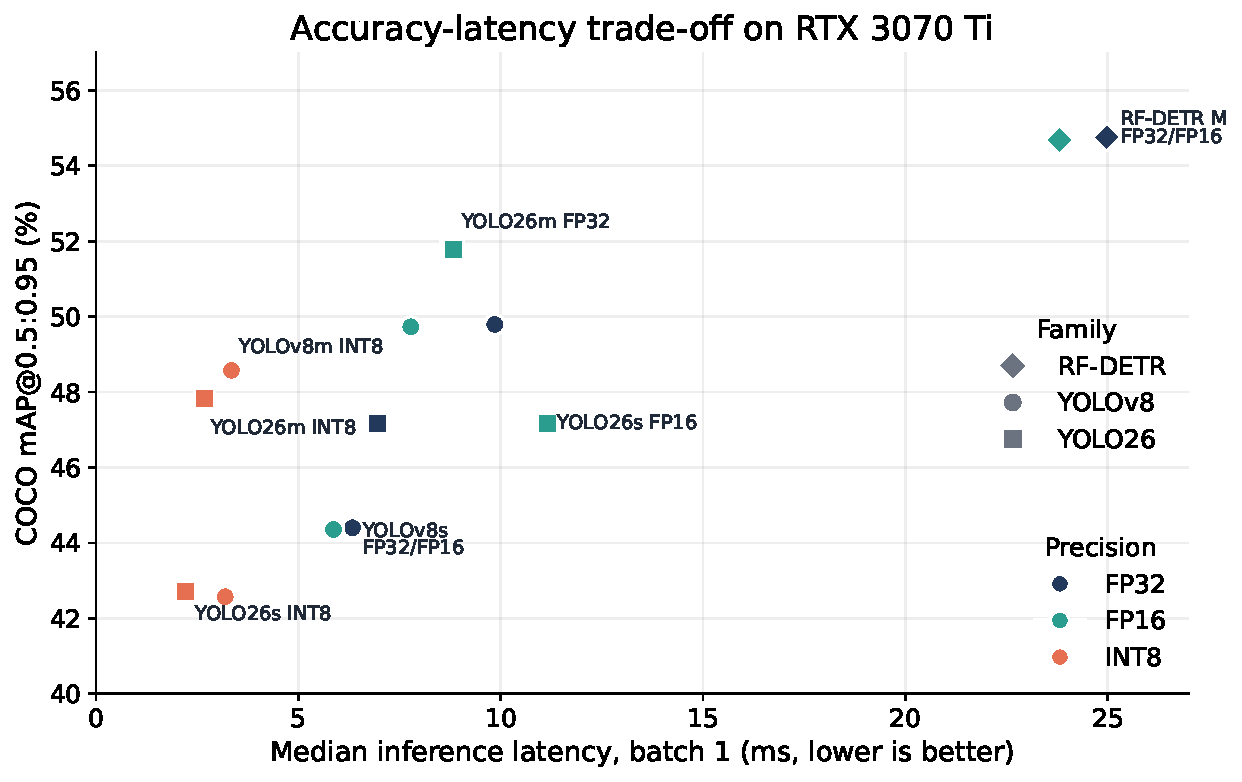
\includegraphics[height=0.82\textheight,width=0.94\linewidth,keepaspectratio]{assets/ap_latency_scatter.pdf}
\noteTime{4:10--6:20. Tell the audience how to read the chart: top-left is better. RF-DETR is the accuracy anchor; YOLO INT8 is the deployment-speed region.}
\end{frame}

% -----------------------------
\begin{frame}{Topline candidates}
\small
\begin{tabular}{l l r r r l}
\toprule
\textbf{Model} & \textbf{Variant} & \textbf{mAP} & \textbf{AP@0.5} & \textbf{Latency} & \textbf{Interpretation}\\
 & & \textbf{(\%)} & \textbf{(\%)} & \textbf{(ms)} & \\
\midrule
RF-DETR M & FP32 & 54.76 & 73.63 & 24.97 & Best accuracy\\
RF-DETR M & FP16 & 54.68 & 73.66 & 23.81 & Same accuracy, lower power\\
YOLO26m & FP32 & 51.80 & 69.06 & 8.76 & Strong YOLO baseline\\
YOLOv8m & INT8 & 48.57 & 65.25 & 3.35 & Best INT8 stability\\
YOLO26m & INT8 & 47.82 & 65.98 & 2.68 & Fast high-accuracy option\\
YOLO26s & INT8 & 42.71 & 59.39 & 2.20 & Fastest measured detector\\
\bottomrule
\end{tabular}

\vspace{3mm}
\textbf{Reading:} if accuracy is the priority, RF-DETR is still ahead. If deployment speed is the priority, TensorRT INT8 YOLO variants move into a much faster latency band.
\noteTime{6:20--7:40. This is the simple table the committee should remember.}
\end{frame}

% -----------------------------
\begin{frame}{RF-DETR evaluation}
\small
\begin{tabular}{l r r r r r}
\toprule
\textbf{Variant} & \textbf{mAP} & \textbf{AP@0.5} & \textbf{Latency} & \textbf{Throughput} & \textbf{Avg. power}\\
 & \textbf{(\%)} & \textbf{(\%)} & \textbf{(ms)} & \textbf{(img/s)} & \textbf{(W)}\\
\midrule
FP32 PyTorch & 54.76 & 73.63 & 24.97 & 40.04 & 136.93\\
FP16 PyTorch & 54.68 & 73.66 & 23.81 & 42.00 & 91.21\\
\bottomrule
\end{tabular}

\vspace{4mm}
\begin{itemize}
  \item FP16 preserves detection quality almost exactly: only 0.08 percentage points of mAP difference.
  \item Latency improves only modestly, from 24.97 ms to 23.81 ms.
  \item Power telemetry improves much more strongly, which makes FP16 still relevant for deployment.
\end{itemize}
\noteTime{7:40--9:00. Explain why this is a useful anchor even though it is slower: it tells us where the accuracy ceiling is.}
\end{frame}

% -----------------------------
\begin{frame}{YOLO FP32 baselines: old vs newer variants}
\small
\begin{tabular}{l r r r r}
\toprule
\textbf{Model} & \textbf{mAP} & \textbf{Latency} & \textbf{Params} & \textbf{FLOPs}\\
 & \textbf{(\%)} & \textbf{(ms)} & \textbf{(M)} & \textbf{(G)}\\
\midrule
YOLOv8s & 44.40 & 6.34 & 11.2 & 28.6\\
YOLO26s & 47.17 & 6.95 & 9.5 & 20.7\\
\midrule
YOLOv8m & 49.79 & 9.86 & 25.9 & 78.9\\
YOLO26m & 51.80 & 8.76 & 20.4 & 68.2\\
\bottomrule
\end{tabular}

\vspace{4mm}
\begin{itemize}
  \item YOLO26m is the strongest YOLO baseline in this run: higher mAP and lower latency than YOLOv8m.
  \item YOLO26s improves accuracy over YOLOv8s with fewer parameters and lower reported FLOPs, but latency is slightly higher.
  \item This confirms that architecture choice changes the deployment trade-off before compression is applied.
\end{itemize}
\noteTime{9:00--10:30. This directly answers why newer YOLO variants were worth adding.}
\end{frame}

% -----------------------------
\begin{frame}{Small YOLO models: YOLOv8s vs YOLO26s}
\small
\begin{tabular}{l r r r r}
\toprule
\textbf{Model} & \textbf{mAP} & \textbf{Latency} & \textbf{Params} & \textbf{FLOPs}\\
 & \textbf{(\%)} & \textbf{(ms)} & \textbf{(M)} & \textbf{(G)}\\
\midrule
YOLOv8s FP32 & 44.40 & 6.34 & 11.2 & 28.6\\
YOLO26s FP32 & 47.17 & 6.95 & 9.5 & 20.7\\
\bottomrule
\end{tabular}

\vspace{4mm}
\begin{itemize}
  \item YOLO26s improves accuracy by 2.77 mAP points over YOLOv8s.
  \item It does this with fewer parameters and lower reported FLOPs.
  \item The latency is slightly worse in this run, showing that FLOPs alone do not predict wall-clock speed.
  \item The small-model result is useful for future pruning because it starts from a compact baseline.
\end{itemize}
\noteTime{10:30--11:30. Do not overclaim: YOLO26s is not simply faster, but it is more accurate and lighter.}
\end{frame}

% -----------------------------
\begin{frame}{Medium YOLO models: YOLOv8m vs YOLO26m}
\small
\begin{tabular}{l r r r r}
\toprule
\textbf{Model} & \textbf{mAP} & \textbf{Latency} & \textbf{Params} & \textbf{FLOPs}\\
 & \textbf{(\%)} & \textbf{(ms)} & \textbf{(M)} & \textbf{(G)}\\
\midrule
YOLOv8m FP32 & 49.79 & 9.86 & 25.9 & 78.9\\
YOLO26m FP32 & 51.80 & 8.76 & 20.4 & 68.2\\
\bottomrule
\end{tabular}

\vspace{4mm}
\begin{itemize}
  \item YOLO26m dominates YOLOv8m in this local run: higher mAP and lower latency.
  \item The improvement is also parameter-efficient: 20.4M parameters versus 25.9M.
  \item This makes YOLO26m the strongest uncompressed YOLO candidate in the current matrix.
  \item It is also a good candidate for QAT or pruning experiments if INT8 PTQ remains too lossy.
\end{itemize}
\noteTime{11:30--12:40. This is one of the strongest current results.}
\end{frame}

% -----------------------------
\begin{frame}{FP16 is not automatically a free win}
\centering
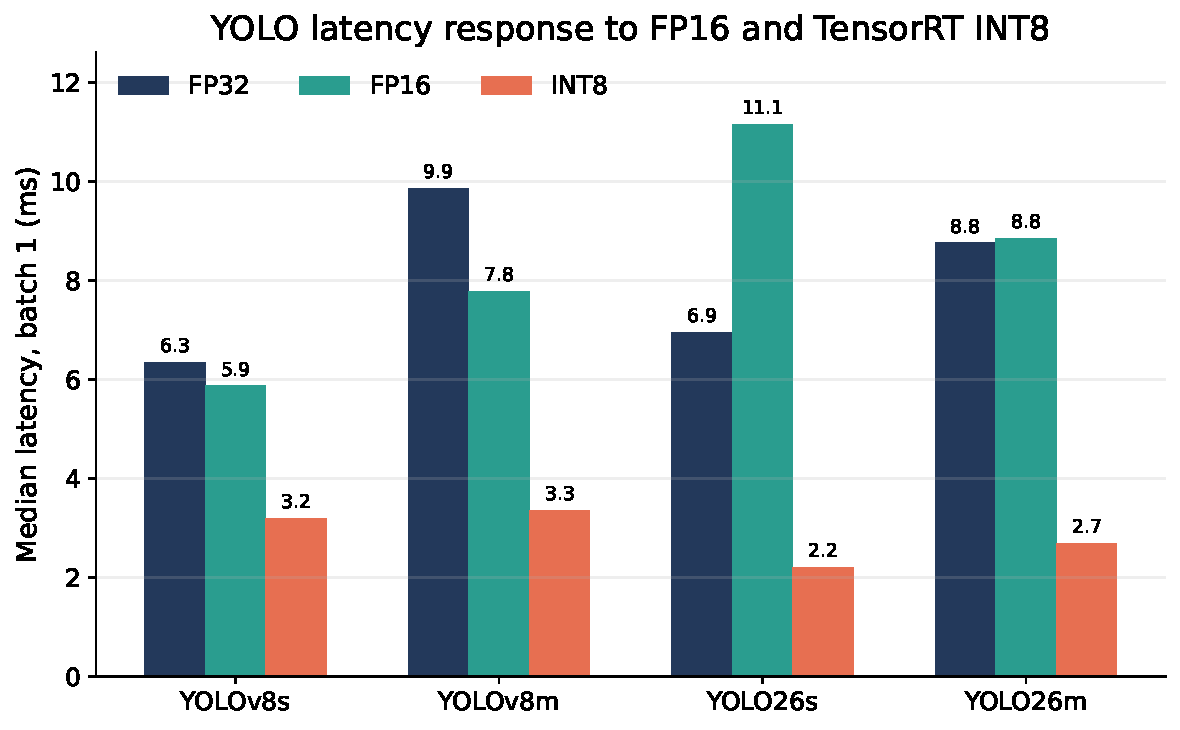
\includegraphics[height=0.79\textheight,width=0.91\linewidth,keepaspectratio]{assets/yolo_latency_by_precision.pdf}

\vspace{1mm}
\footnotesize INT8 uses TensorRT; FP32 and FP16 use the PyTorch/Ultralytics path.
\noteTime{10:30--12:00. Key message: FP16 helped YOLOv8m, barely helped or hurt YOLO26. Runtime implementation matters.}
\end{frame}

% -----------------------------
\begin{frame}{Accuracy under precision changes}
\centering
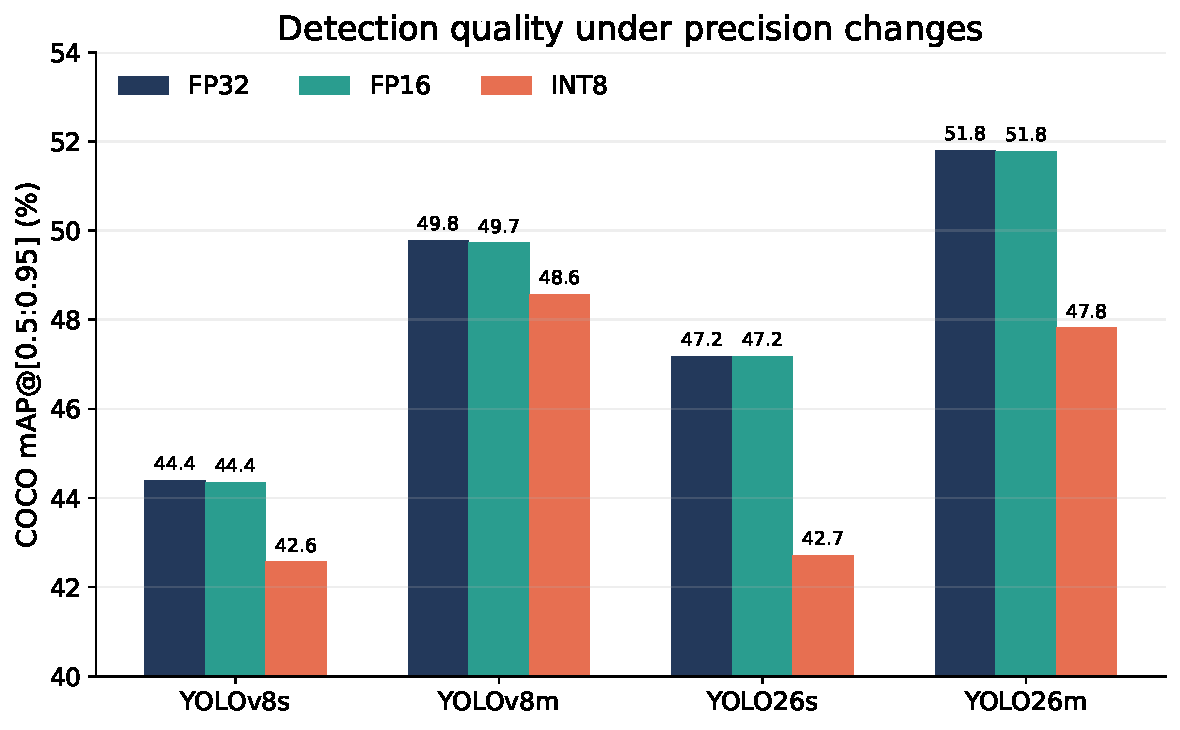
\includegraphics[height=0.79\textheight,width=0.91\linewidth,keepaspectratio]{assets/yolo_ap_by_precision.pdf}

\vspace{1mm}
\footnotesize FP16 preserves mAP; INT8 PTQ has an architecture-dependent accuracy cost.
\noteTime{12:00--13:30. FP16 keeps accuracy. INT8 has an accuracy cost, and the cost differs strongly by architecture.}
\end{frame}

% -----------------------------
\begin{frame}{INT8 PTQ trade-off}
\begin{columns}[T,onlytextwidth]
\begin{column}{0.57\textwidth}
\centering
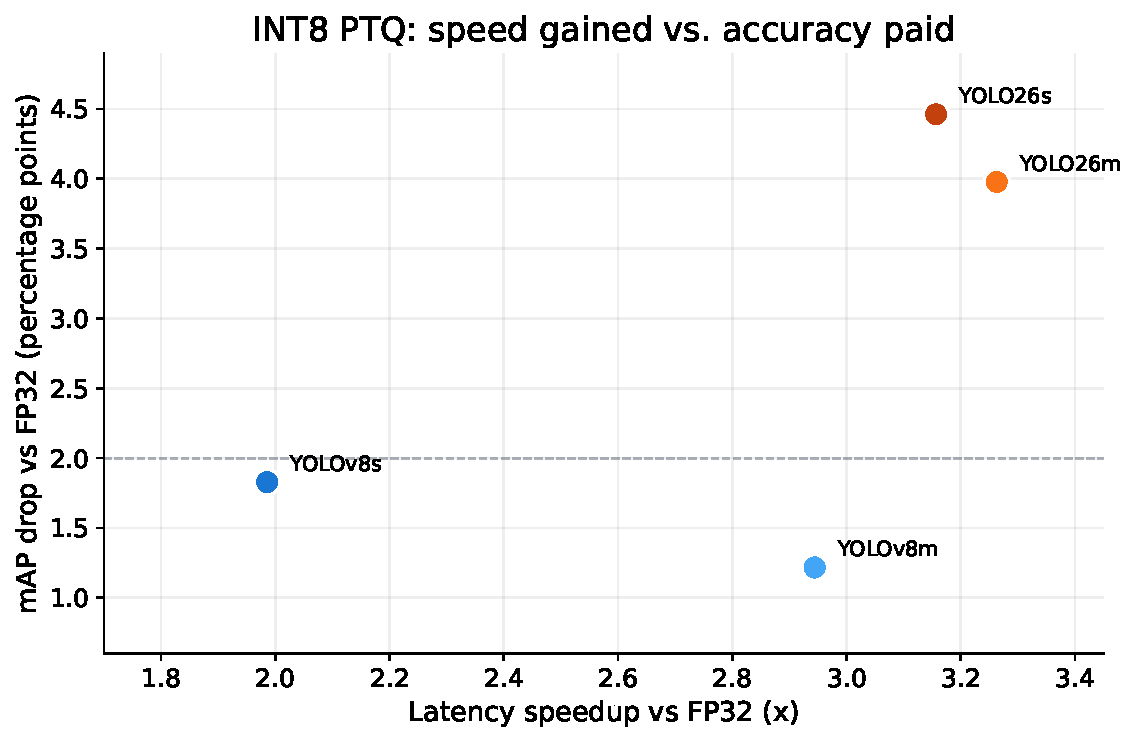
\includegraphics[width=\linewidth]{assets/int8_speed_accuracy_tradeoff.pdf}

\vspace{1mm}
\footnotesize INT8 speedup versus mAP loss relative to each FP32 baseline.
\end{column}
\begin{column}{0.40\textwidth}
\small
\begin{tabular}{l r r}
\toprule
\textbf{Model} & \textbf{Speedup} & \textbf{mAP loss}\\
 & \textbf{(x)} & \textbf{(pp)}\\
\midrule
YOLOv8s & 1.99 & 1.83\\
YOLOv8m & 2.94 & 1.22\\
YOLO26s & 3.16 & 4.46\\
YOLO26m & 3.26 & 3.98\\
\bottomrule
\end{tabular}

\vspace{3mm}
\textbf{Interpretation:} YOLOv8m is the most robust to PTQ, while YOLO26 gains more latency but pays a larger mAP cost.
\end{column}
\end{columns}
\noteTime{13:30--15:20. Emphasise that this is exactly the compression trade-off the thesis studies.}
\end{frame}

% -----------------------------
\begin{frame}{Best candidates by deployment priority}
\small
\begin{tabular}{>{\raggedright\arraybackslash}p{0.20\textwidth}>{\raggedright\arraybackslash}p{0.28\textwidth}>{\raggedright\arraybackslash}p{0.42\textwidth}}
\toprule
\textbf{Priority} & \textbf{Candidate} & \textbf{Reason}\\
\midrule
Maximum accuracy & RF-DETR M FP16\newline 54.68 mAP, 23.81 ms & Highest quality; FP16 reduces power with almost no accuracy loss.\\
Balanced YOLO & YOLO26m FP32\newline 51.80 mAP, 8.76 ms & Best uncompressed YOLO trade-off in the current run.\\
Robust INT8 & YOLOv8m INT8\newline 48.57 mAP, 3.35 ms & Lowest mAP loss from PTQ among the YOLO INT8 variants.\\
Fast INT8 & YOLO26m INT8\newline 47.82 mAP, 2.68 ms & Strong speed with still competitive AP@0.5.\\
Fastest measured & YOLO26s INT8\newline 42.71 mAP, 2.20 ms & Lowest latency, but the accuracy cost is larger.\\
\bottomrule
\end{tabular}

\vspace{3mm}
\textbf{Thesis implication:} there is no single winner; the best choice depends on whether the target optimises for accuracy, speed, or robustness to quantisation.
\noteTime{15:20--16:20. This slide gives a decision-oriented summary before the hypothesis evaluation.}
\end{frame}

% -----------------------------
\begin{frame}{Evaluation against the research hypotheses}
\begin{itemize}
  \item \textbf{Precision compression improves deployment speed.}\\
  Confirmed for TensorRT INT8 YOLO: roughly 2.0x--3.3x lower latency with measurable but bounded mAP loss.
  \item \textbf{Architecture affects compression behaviour.}\\
  Confirmed: YOLOv8m loses only 1.22 pp mAP under INT8, while YOLO26m loses 3.98 pp despite being faster.
  \item \textbf{Transformer-style detectors need token/runtime compression, not only FP16.}\\
  Partially supported: RF-DETR has the best accuracy, but FP16 alone does not change latency enough.
  \item \textbf{Ordering effects and pruning/token reduction still need experimental evidence.}\\
  Not yet tested; this is the next ablation stage after the baseline precision grid.
\end{itemize}
\noteTime{15:20--17:00. This slide converts measurements into thesis claims.}
\end{frame}

% -----------------------------
\begin{frame}{Current limitations}
\begin{itemize}
  \item Swin-T Mask R-CNN is not yet evaluated because MMDetection/MMCV setup is unstable on native Windows with the current Python/CUDA stack.
  \item RF-DETR INT8 PTQ is queued, but requires an ONNX/TensorRT export path before it can be measured fairly.
  \item INT8 results use post-training quantisation with a 500-image calibration subset; QAT may recover accuracy, especially for YOLO26.
  \item Power and energy telemetry are useful early indicators, but final claims should be based on repeated runs after the workflow metadata fix.
  \item The RTX 3070 Ti is the current target hardware; final edge-device claims should distinguish GPU-local results from embedded deployment.
\end{itemize}
\noteTime{17:00--18:30. Be transparent. This protects the thesis and shows you know what remains unresolved.}
\end{frame}

% -----------------------------
\begin{frame}{Next experiments}
\begin{enumerate}
  \item Re-run the overnight profile after the image-count metadata fix and freeze the curated result table.
  \item Complete Swin-T evaluation in a compatible WSL2/Linux OpenMMLab environment.
  \item Add RF-DETR ONNX/TensorRT export, then test INT8 PTQ.
  \item Implement one conservative token-reduction setting for RF-DETR/Swin and compare actual latency, not only FLOPs.
  \item Add one structured-pruning YOLO ablation and then test pruning + INT8 ordering.
  \item Optional robustness check: blur, noise, and JPEG degradation for FP32 versus INT8 detectors.
\end{enumerate}
\noteTime{18:30--20:00. Finish by showing the remaining work is scoped, not vague.}
\end{frame}

% -----------------------------
\begin{frame}{Conclusion}
\Large
\textbf{The preliminary results already support the thesis direction: compression is useful, but the best method depends strongly on architecture and runtime.}

\vspace{7mm}
\normalsize
\begin{itemize}
  \item RF-DETR currently defines the accuracy ceiling: 54.8 mAP at about 25 ms.
  \item YOLO26m is the strongest dense-detector baseline before compression.
  \item TensorRT INT8 gives the largest deployment-speed gains, especially for YOLO, but the accuracy cost is architecture-dependent.
\end{itemize}
\noteTime{20:00--20:40. Leave time for questions.}
\end{frame}

\end{document}
